% IEEE standard conference template; to be used with:
%   spconf.sty  - LaTeX style file, and
%   IEEEbib.bst - IEEE bibliography style file.
% --------------------------------------------------------------------------

\documentclass[letterpaper]{article}
\usepackage{spconf,amsmath,amssymb,graphicx,float,enumitem,url,algpseudocode}

% Example definitions.
% --------------------
% nice symbols for real and complex numbers
\newcommand{\R}[0]{\mathbb{R}}
\newcommand{\C}[0]{\mathbb{C}}

% bold paragraph titles
\newcommand{\mypar}[1]{{\bf #1.}}

% Title.
% ------
\title{Optimization and parallelization of diffusion solvers\\
using alternating direction implicit and random walk methods}
%
% Single address.
% ---------------
\name{Samuel Maloney} 
\address{Department of Mathematics\\ETH Z\"urich\\Z\"urich, Switzerland}

% For example:
% ------------
%\address{School\\
%		 Department\\
%		 Address}
%
% Two addresses (uncomment and modify for two-address case).
% ----------------------------------------------------------
%\twoauthors
%  {A. Author-one, B. Author-two\sthanks{Thanks to XYZ agency for funding.}}
%		 {School A-B\\
%		 Department A-B\\
%		 Address A-B}
%  {C. Author-three, D. Author-four\sthanks{The fourth author performed the work
%		 while at ...}}
%		 {School C-D\\
%		 Department C-D\\
%		 Address C-D}
%

\begin{document}
%\ninept
%
\maketitle
%


% ----------------------------------------------------------------------
\begin{abstract}
An optimized code for diffusion is presented. 
\end{abstract}


% ----------------------------------------------------------------------
\section{Background}\label{sec:background}

\mypar{Motivation} 
Diffusion is the process by which a~quantity of interest spreads from regions of high density to regions of low density and are integral in the study of fluids. Diffusion terms arise in all numerical models of computational fluid dynamics, which are used for such problems as aerodynamic design, turbine flows, chemical reaction mixing, and many others. Efficient and accurate simulation codes for diffusion are thus of great importance in many fields.

In this study, two different algorithms to simulate the diffusion process, Alternating Direction Implicit (ADI) and a Random Walk (RW), were implemented, optimized, and parallelized. The mathematical formulations for diffusion in general and for each of these two methods specifically are presented next.

\mypar{Mathematical Formulation}
The process of diffusion is driven by it's conentration gradient according to the diffusion equation:
\begin{equation}
\frac{\partial \rho(\mathbf{r},t)}{\partial t} = D\Delta\rho(\mathbf{r},t)
\end{equation}
where $\rho(\mathbf{r},t)$, with position $\mathbf{r}$ at time $t$, is the quantity of interest and $D$ is the diffusion constant and is a given value for the system. For this study, homogeneous Dirichlet boundary conditions are used at all boundaries. The initial density distribution used for this study is:
\begin{equation}
\rho(x,y,0)=\sin(\pi x)\sin(\pi y)
\end{equation}
and it's corresponding analytic solution, which was used for verification, is:
\begin{equation}
\rho(x,y,t)=\sin(\pi x)\sin(\pi y)e^{-2D\pi^{2}t}
\end{equation}
The studied simulation domain is a unit square with $x$ and $y$ each ranging from $0$ to $1$, which is discretized using a uniform grid such that $\delta h=\delta x=\delta y$. A superscript $n$ is used to denote the timestep $t_n=n\delta t$ and subscripts $i$ and $j$ to denote the indices of the nodes in the mesh $x_i=i\delta x$ and $y_j=j\delta y$ such that $\rho_{i,j}^{n}=\rho(x_i,y_j,t_n)$.

\mypar{Alternating Direction Implicit}
Lorem Ipsum dolor sit amet.

\mypar{Random Walk}
Lorem Ipsum dolor sit amet.

% ----------------------------------------------------------------------
\section{Baseline Implementation}\label{sec:baseline}

In this section, we provide an overview of the algorithm 

\mypar{ADI}
Lorem Ipsum dolor sit amet.

\mypar{RW}
Lorem Ipsum dolor sit amet.

\mypar{Cost Analysis}
We define the cost of the code as the number of floating point operations (FLOPs) including additions, multiplications, and, for the ADI baseline implementation only, divisions. Moreover, the data movement in bytes to and from various levels of cache was measured in order to quantify the operational intensity.

The ADI complexity is roughly $O(N^2)$ as it does a constant number of operations for calculating the updated value at each point in the grid.

Scaling for the RW method depends on which version is being considered. The baseline implementation scales as $O(M)$, where $M$ is the number of particles in the simulation. This is because a random number must be generated for each particle in the simulation to determine it's movement for a given timestep, independent of how many grid points there are in the simulation. The later versions that use a binomial random variable (see \ref{subsec:RW_method}) to simulate particle movement scale as $O(N^2)$ because exactly four such random variables must be evaluated for each grid point, independent of the number of particles in the simulation.


% ----------------------------------------------------------------------
\section{Optimization Method}\label{sec:method}

In this section we explain the main optimizations that were undertaken.
We discuss the optimizations of the ADI and RW methods in separate subsections.

\subsection{ADI}\label{subsec:ADI_method}

We divide the optimizations in 4 sets called \textit{revisions}.

\mypar{Scalar}
This revision consists mainly of 

\mypar{AVX}
In this revision we used

\mypar{OpenMP}
This revision was targeted at 


\subsection{RW}\label{subsec:RW_method}

TheRW optimizations can be similarly broken down into revisions, simlarily to those for the assembly.

\mypar{Scalar}
This is a direct implentation

\mypar{AVX}
Vectorization of the code was done by leveraging Intel fused-multiply-add (FMA) and advanced vector extension (AVX) intrinsics.

\mypar{OpenMP}
stuff...


% ----------------------------------------------------------------------
\section{Optimization Results}\label{sec:results}

In this section the results of numerical benchmarks of the code at various stages are presented. Runtime, performance, and roofline analyses were performed where applicable.

\mypar{Experimental setup}
All data was collected using a single XC50 node of Piz Daint, which has a 12 core Intel Xeon E5-2690 v3 running at 2.6 GHz \cite{daint}. Each physical processor core has a 64 KB L1 cache split equally into two 32 KB data and instruction caches, and a 256 KB unified L2 cache \cite{cpu_world}. The 30 MB L3 cache is shared between all cores \cite{ark_intel}, and there is 24.9 GB/s bandwidth to main memory \cite{7_cpu}. The Intel C++ Compiler v17.0.1 was used with "-O3 -std=c++11 -DNDEBUG -march=core-avx2 -fno-alias -qopenmp -mkl" flags. The Intel time stamp counter (TSC) was used for runtime measurements and CrayPat was used for cache miss measurements.

The inputs are the number of grid points in domain discretization, the time stepbetween iterations, and the number of iterations performed. We used grids of various sizes, up to $N\times N=7680\times7680$. The diffusion constant $D=1$ is used for all simulations. All experiments were performed with warm cache.

\subsection{ADI}\label{subsec:ADI_results}
Roofline, runtime, and scaling experiments were conducted on the ADI code.

\mypar{Results}
The runtime plots of various revisions of the ADI code (see \ref{subsec:ADI_method}) are shown in Fig. \ref{fig:runtime_assemby}. Each consecutive revision of the code resulted in a~speedup.

\begin{figure}\centering
  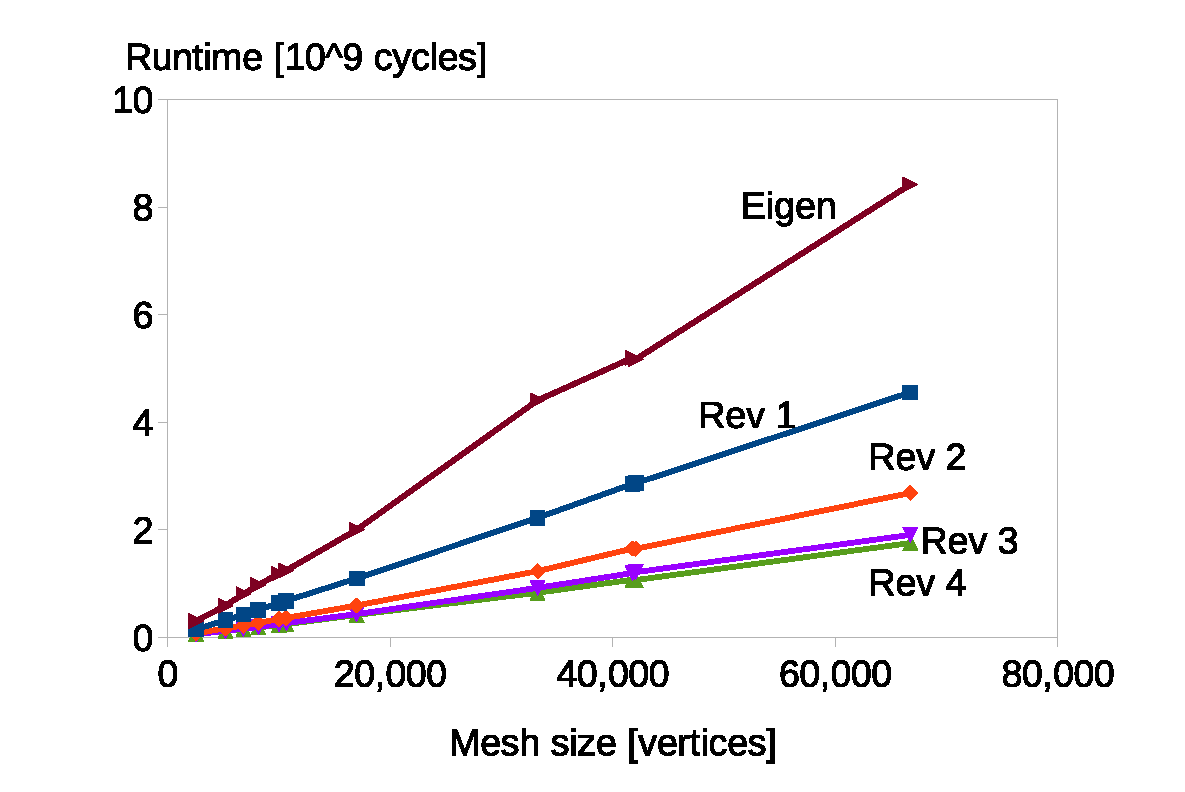
\includegraphics[width=\linewidth]{./plots/assembly_runtime.eps}
  \caption{Runtime analysis of the matrix assembly code.}
  \label{fig:runtime_assemby}
\end{figure}

\subsection{RW}\label{subsec:RW_results}
Benchmarking experiments were conducted on the RW code

\mypar{Results}
Results of the roofline, performance, and runtime analyses of the RW code will now be presented.


% ----------------------------------------------------------------------
\section{Conclusion}
Conclude things

% ----------------------------------------------------------------------


\begin{thebibliography}{99}

\urlstyle{same}

\bibitem{daint}{CSCS. (Accessed 2017, Aug). \emph{Piz Daint} [Online]. Available: \url{http://www.cscs.ch/computers/piz_daint/}}

\bibitem{cpu_world}{CPU-World. (Accessed 2017, Aug). \emph{Intel Xeon E5-2690 v3 specifications} [Online]. Available: \url{http://www.cpu-world.com/CPUs/Xeon/Intel-Xeon%20E5-2690%20v3.html}}

\bibitem{ark_intel}{Intel Corporation. (Accessed 2017, Aug). \emph{Intel Xeon Processor E5-2690 v3} [Online]. Available: \url{http://ark.intel.com/products/81713/Intel-Xeon-Processor-E5-2690-v3-30M-Cache-2_60-GHzl}}

\bibitem{7_cpu}{7-CPU. (Accessed 2017, Aug). \emph{Intel Haswell} [Online]. Available: \url{http://www.7-cpu.com/cpu/Haswell.html}}

\bibitem{transpose}{user2927848. (2016, Mar 23). \emph{m256d TRANSPOSE4 Equivalent} [Online]. Available: \url{https://stackoverflow.com/questions/36167517/m256d-transpose4-equivalent}}

\bibitem{sitmo}{T. van den Berg. (Accessed 2017, Aug). \emph{High Quality C++ Parallel Random Number Generator} [Online]. Available: \url{https://www.sitmo.com/?p=1206}}

\bibitem{manual_intel}{Intel Corporation. (2016, Jun). \emph{Intel 64 and IA-32 Architectures Optimization Reference Manual} [Online]. Available: \url{https://www.intel.com/content/www/us/en/architecture-and-technology/64-ia-32-architectures-optimization-manual.html}}

\end{thebibliography}

\end{document}
